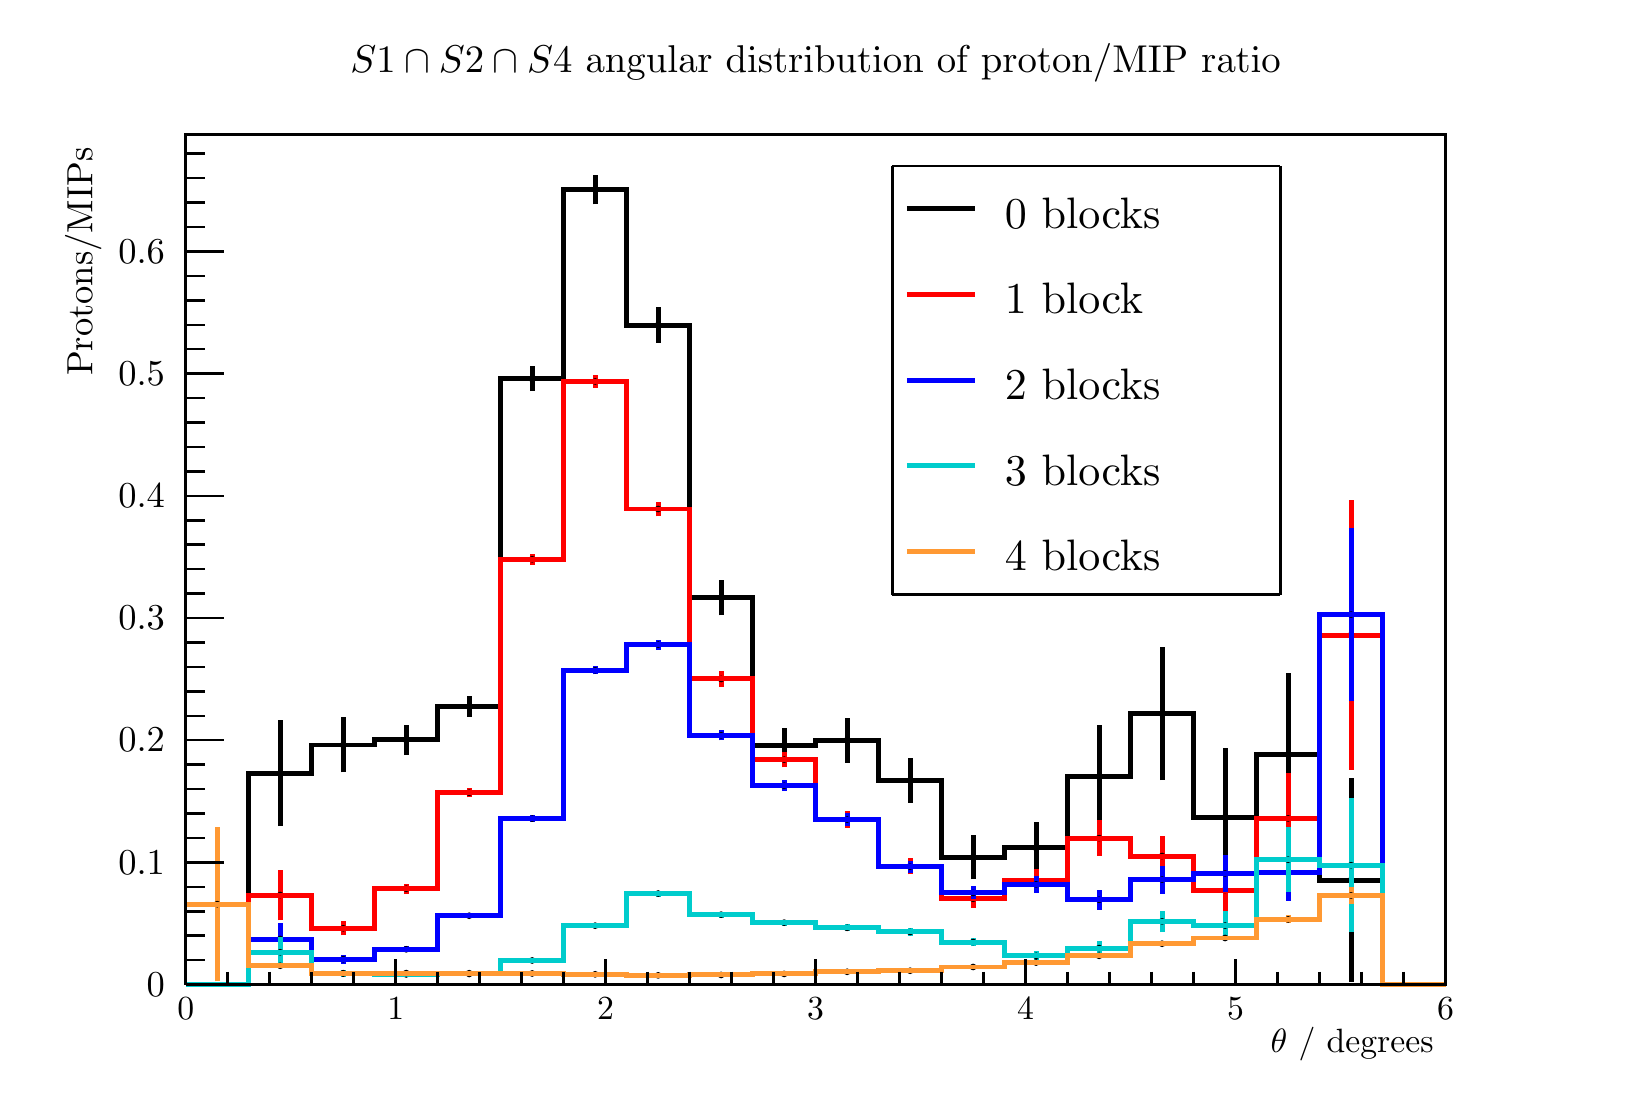
\begin{tikzpicture}
\pgfdeclareplotmark{cross} {
\pgfpathmoveto{\pgfpoint{-0.3\pgfplotmarksize}{\pgfplotmarksize}}
\pgfpathlineto{\pgfpoint{+0.3\pgfplotmarksize}{\pgfplotmarksize}}
\pgfpathlineto{\pgfpoint{+0.3\pgfplotmarksize}{0.3\pgfplotmarksize}}
\pgfpathlineto{\pgfpoint{+1\pgfplotmarksize}{0.3\pgfplotmarksize}}
\pgfpathlineto{\pgfpoint{+1\pgfplotmarksize}{-0.3\pgfplotmarksize}}
\pgfpathlineto{\pgfpoint{+0.3\pgfplotmarksize}{-0.3\pgfplotmarksize}}
\pgfpathlineto{\pgfpoint{+0.3\pgfplotmarksize}{-1.\pgfplotmarksize}}
\pgfpathlineto{\pgfpoint{-0.3\pgfplotmarksize}{-1.\pgfplotmarksize}}
\pgfpathlineto{\pgfpoint{-0.3\pgfplotmarksize}{-0.3\pgfplotmarksize}}
\pgfpathlineto{\pgfpoint{-1.\pgfplotmarksize}{-0.3\pgfplotmarksize}}
\pgfpathlineto{\pgfpoint{-1.\pgfplotmarksize}{0.3\pgfplotmarksize}}
\pgfpathlineto{\pgfpoint{-0.3\pgfplotmarksize}{0.3\pgfplotmarksize}}
\pgfpathclose
\pgfusepathqstroke
}
\pgfdeclareplotmark{cross*} {
\pgfpathmoveto{\pgfpoint{-0.3\pgfplotmarksize}{\pgfplotmarksize}}
\pgfpathlineto{\pgfpoint{+0.3\pgfplotmarksize}{\pgfplotmarksize}}
\pgfpathlineto{\pgfpoint{+0.3\pgfplotmarksize}{0.3\pgfplotmarksize}}
\pgfpathlineto{\pgfpoint{+1\pgfplotmarksize}{0.3\pgfplotmarksize}}
\pgfpathlineto{\pgfpoint{+1\pgfplotmarksize}{-0.3\pgfplotmarksize}}
\pgfpathlineto{\pgfpoint{+0.3\pgfplotmarksize}{-0.3\pgfplotmarksize}}
\pgfpathlineto{\pgfpoint{+0.3\pgfplotmarksize}{-1.\pgfplotmarksize}}
\pgfpathlineto{\pgfpoint{-0.3\pgfplotmarksize}{-1.\pgfplotmarksize}}
\pgfpathlineto{\pgfpoint{-0.3\pgfplotmarksize}{-0.3\pgfplotmarksize}}
\pgfpathlineto{\pgfpoint{-1.\pgfplotmarksize}{-0.3\pgfplotmarksize}}
\pgfpathlineto{\pgfpoint{-1.\pgfplotmarksize}{0.3\pgfplotmarksize}}
\pgfpathlineto{\pgfpoint{-0.3\pgfplotmarksize}{0.3\pgfplotmarksize}}
\pgfpathclose
\pgfusepathqfillstroke
}
\pgfdeclareplotmark{newstar} {
\pgfpathmoveto{\pgfqpoint{0pt}{\pgfplotmarksize}}
\pgfpathlineto{\pgfqpointpolar{44}{0.5\pgfplotmarksize}}
\pgfpathlineto{\pgfqpointpolar{18}{\pgfplotmarksize}}
\pgfpathlineto{\pgfqpointpolar{-20}{0.5\pgfplotmarksize}}
\pgfpathlineto{\pgfqpointpolar{-54}{\pgfplotmarksize}}
\pgfpathlineto{\pgfqpointpolar{-90}{0.5\pgfplotmarksize}}
\pgfpathlineto{\pgfqpointpolar{234}{\pgfplotmarksize}}
\pgfpathlineto{\pgfqpointpolar{198}{0.5\pgfplotmarksize}}
\pgfpathlineto{\pgfqpointpolar{162}{\pgfplotmarksize}}
\pgfpathlineto{\pgfqpointpolar{134}{0.5\pgfplotmarksize}}
\pgfpathclose
\pgfusepathqstroke
}
\pgfdeclareplotmark{newstar*} {
\pgfpathmoveto{\pgfqpoint{0pt}{\pgfplotmarksize}}
\pgfpathlineto{\pgfqpointpolar{44}{0.5\pgfplotmarksize}}
\pgfpathlineto{\pgfqpointpolar{18}{\pgfplotmarksize}}
\pgfpathlineto{\pgfqpointpolar{-20}{0.5\pgfplotmarksize}}
\pgfpathlineto{\pgfqpointpolar{-54}{\pgfplotmarksize}}
\pgfpathlineto{\pgfqpointpolar{-90}{0.5\pgfplotmarksize}}
\pgfpathlineto{\pgfqpointpolar{234}{\pgfplotmarksize}}
\pgfpathlineto{\pgfqpointpolar{198}{0.5\pgfplotmarksize}}
\pgfpathlineto{\pgfqpointpolar{162}{\pgfplotmarksize}}
\pgfpathlineto{\pgfqpointpolar{134}{0.5\pgfplotmarksize}}
\pgfpathclose
\pgfusepathqfillstroke
}
\definecolor{c}{rgb}{1,1,1};
\draw [color=c, fill=c] (0,0) rectangle (20,13.4957);
\draw [color=c, fill=c] (2,1.34957) rectangle (18,12.1461);
\definecolor{c}{rgb}{0,0,0};
\draw [c,line width=0.9] (2,1.34957) -- (2,12.1461) -- (18,12.1461) -- (18,1.34957) -- (2,1.34957);
\definecolor{c}{rgb}{1,1,1};
\draw [color=c, fill=c] (2,1.34957) rectangle (18,12.1461);
\definecolor{c}{rgb}{0,0,0};
\draw [c,line width=0.9] (2,1.34957) -- (2,12.1461) -- (18,12.1461) -- (18,1.34957) -- (2,1.34957);
\definecolor{c}{rgb}{0,0,0.6};
\draw [c,line width=0.9] (2,1.34957) -- (2.8,1.34957) -- (2.8,1.34957) -- (3.6,1.34957) -- (3.6,1.34957) -- (4.4,1.34957) -- (4.4,1.34957) -- (5.2,1.34957) -- (5.2,1.34957) -- (6,1.34957) -- (6,1.34957) -- (6.8,1.34957) -- (6.8,1.34957) --
 (7.6,1.34957) -- (7.6,1.34957) -- (8.4,1.34957) -- (8.4,1.34957) -- (9.2,1.34957) -- (9.2,1.34957) -- (10,1.34957) -- (10,1.34957) -- (10.8,1.34957) -- (10.8,1.34957) -- (11.6,1.34957) -- (11.6,1.34957) -- (12.4,1.34957) -- (12.4,1.34957) --
 (13.2,1.34957) -- (13.2,1.34957) -- (14,1.34957) -- (14,1.34957) -- (14.8,1.34957) -- (14.8,1.34957) -- (15.6,1.34957) -- (15.6,1.34957) -- (16.4,1.34957) -- (16.4,1.34957) -- (17.2,1.34957) -- (17.2,1.34957) -- (18,1.34957);
\definecolor{c}{rgb}{0,0,0};
\draw [c,line width=0.9] (2,1.34957) -- (18,1.34957);
\draw [c,line width=0.9] (2,1.67347) -- (2,1.34957);
\draw [c,line width=0.9] (2.53333,1.51152) -- (2.53333,1.34957);
\draw [c,line width=0.9] (3.06667,1.51152) -- (3.06667,1.34957);
\draw [c,line width=0.9] (3.6,1.51152) -- (3.6,1.34957);
\draw [c,line width=0.9] (4.13333,1.51152) -- (4.13333,1.34957);
\draw [c,line width=0.9] (4.66667,1.67347) -- (4.66667,1.34957);
\draw [c,line width=0.9] (5.2,1.51152) -- (5.2,1.34957);
\draw [c,line width=0.9] (5.73333,1.51152) -- (5.73333,1.34957);
\draw [c,line width=0.9] (6.26667,1.51152) -- (6.26667,1.34957);
\draw [c,line width=0.9] (6.8,1.51152) -- (6.8,1.34957);
\draw [c,line width=0.9] (7.33333,1.67347) -- (7.33333,1.34957);
\draw [c,line width=0.9] (7.86667,1.51152) -- (7.86667,1.34957);
\draw [c,line width=0.9] (8.4,1.51152) -- (8.4,1.34957);
\draw [c,line width=0.9] (8.93333,1.51152) -- (8.93333,1.34957);
\draw [c,line width=0.9] (9.46667,1.51152) -- (9.46667,1.34957);
\draw [c,line width=0.9] (10,1.67347) -- (10,1.34957);
\draw [c,line width=0.9] (10.5333,1.51152) -- (10.5333,1.34957);
\draw [c,line width=0.9] (11.0667,1.51152) -- (11.0667,1.34957);
\draw [c,line width=0.9] (11.6,1.51152) -- (11.6,1.34957);
\draw [c,line width=0.9] (12.1333,1.51152) -- (12.1333,1.34957);
\draw [c,line width=0.9] (12.6667,1.67347) -- (12.6667,1.34957);
\draw [c,line width=0.9] (13.2,1.51152) -- (13.2,1.34957);
\draw [c,line width=0.9] (13.7333,1.51152) -- (13.7333,1.34957);
\draw [c,line width=0.9] (14.2667,1.51152) -- (14.2667,1.34957);
\draw [c,line width=0.9] (14.8,1.51152) -- (14.8,1.34957);
\draw [c,line width=0.9] (15.3333,1.67347) -- (15.3333,1.34957);
\draw [c,line width=0.9] (15.8667,1.51152) -- (15.8667,1.34957);
\draw [c,line width=0.9] (16.4,1.51152) -- (16.4,1.34957);
\draw [c,line width=0.9] (16.9333,1.51152) -- (16.9333,1.34957);
\draw [c,line width=0.9] (17.4667,1.51152) -- (17.4667,1.34957);
\draw [c,line width=0.9] (18,1.67347) -- (18,1.34957);
\draw [anchor=base] (2,0.904212) node[scale=1.21821, color=c, rotate=0]{0};
\draw [anchor=base] (4.66667,0.904212) node[scale=1.21821, color=c, rotate=0]{1};
\draw [anchor=base] (7.33333,0.904212) node[scale=1.21821, color=c, rotate=0]{2};
\draw [anchor=base] (10,0.904212) node[scale=1.21821, color=c, rotate=0]{3};
\draw [anchor=base] (12.6667,0.904212) node[scale=1.21821, color=c, rotate=0]{4};
\draw [anchor=base] (15.3333,0.904212) node[scale=1.21821, color=c, rotate=0]{5};
\draw [anchor=base] (18,0.904212) node[scale=1.21821, color=c, rotate=0]{6};
\draw [anchor= east] (18,0.593811) node[scale=1.21821, color=c, rotate=0]{$\theta$ / degrees};
\draw [c,line width=0.9] (2,1.34957) -- (2,12.1461);
\draw [c,line width=0.9] (2.48,1.34957) -- (2,1.34957);
\draw [c,line width=0.9] (2.24,1.65993) -- (2,1.65993);
\draw [c,line width=0.9] (2.24,1.97029) -- (2,1.97029);
\draw [c,line width=0.9] (2.24,2.28066) -- (2,2.28066);
\draw [c,line width=0.9] (2.24,2.59102) -- (2,2.59102);
\draw [c,line width=0.9] (2.48,2.90138) -- (2,2.90138);
\draw [c,line width=0.9] (2.24,3.21174) -- (2,3.21174);
\draw [c,line width=0.9] (2.24,3.5221) -- (2,3.5221);
\draw [c,line width=0.9] (2.24,3.83247) -- (2,3.83247);
\draw [c,line width=0.9] (2.24,4.14283) -- (2,4.14283);
\draw [c,line width=0.9] (2.48,4.45319) -- (2,4.45319);
\draw [c,line width=0.9] (2.24,4.76355) -- (2,4.76355);
\draw [c,line width=0.9] (2.24,5.07391) -- (2,5.07391);
\draw [c,line width=0.9] (2.24,5.38428) -- (2,5.38428);
\draw [c,line width=0.9] (2.24,5.69464) -- (2,5.69464);
\draw [c,line width=0.9] (2.48,6.005) -- (2,6.005);
\draw [c,line width=0.9] (2.24,6.31536) -- (2,6.31536);
\draw [c,line width=0.9] (2.24,6.62572) -- (2,6.62572);
\draw [c,line width=0.9] (2.24,6.93609) -- (2,6.93609);
\draw [c,line width=0.9] (2.24,7.24645) -- (2,7.24645);
\draw [c,line width=0.9] (2.48,7.55681) -- (2,7.55681);
\draw [c,line width=0.9] (2.24,7.86717) -- (2,7.86717);
\draw [c,line width=0.9] (2.24,8.17753) -- (2,8.17753);
\draw [c,line width=0.9] (2.24,8.4879) -- (2,8.4879);
\draw [c,line width=0.9] (2.24,8.79826) -- (2,8.79826);
\draw [c,line width=0.9] (2.48,9.10862) -- (2,9.10862);
\draw [c,line width=0.9] (2.24,9.41898) -- (2,9.41898);
\draw [c,line width=0.9] (2.24,9.72934) -- (2,9.72934);
\draw [c,line width=0.9] (2.24,10.0397) -- (2,10.0397);
\draw [c,line width=0.9] (2.24,10.3501) -- (2,10.3501);
\draw [c,line width=0.9] (2.48,10.6604) -- (2,10.6604);
\draw [c,line width=0.9] (2.48,10.6604) -- (2,10.6604);
\draw [c,line width=0.9] (2.24,10.9708) -- (2,10.9708);
\draw [c,line width=0.9] (2.24,11.2812) -- (2,11.2812);
\draw [c,line width=0.9] (2.24,11.5915) -- (2,11.5915);
\draw [c,line width=0.9] (2.24,11.9019) -- (2,11.9019);
\draw [anchor= east] (1.9,1.34957) node[scale=1.31821, color=c, rotate=0]{0};
\draw [anchor= east] (1.9,2.90138) node[scale=1.31821, color=c, rotate=0]{0.1};
\draw [anchor= east] (1.9,4.45319) node[scale=1.31821, color=c, rotate=0]{0.2};
\draw [anchor= east] (1.9,6.005) node[scale=1.31821, color=c, rotate=0]{0.3};
\draw [anchor= east] (1.9,7.55681) node[scale=1.31821, color=c, rotate=0]{0.4};
\draw [anchor= east] (1.9,9.10862) node[scale=1.31821, color=c, rotate=0]{0.5};
\draw [anchor= east] (1.9,10.6604) node[scale=1.31821, color=c, rotate=0]{0.6};
\draw [anchor= east] (0.698281,12.1461) node[scale=1.31821, color=c, rotate=90]{ Protons/MIPs};
\draw [c,line width=1.8] (3.2,3.36179) -- (3.2,4.03295);
\draw [c,line width=1.8] (3.2,4.03295) -- (3.2,4.70411);
\foreach \P in {(3.2,4.03295)}{\draw[mark options={color=c,fill=c},mark size=2.402402pt,mark=*,mark size=1pt] plot coordinates {\P};}
\draw [c,line width=1.8] (4,4.04344) -- (4,4.39272);
\draw [c,line width=1.8] (4,4.39272) -- (4,4.74201);
\foreach \P in {(4,4.39272)}{\draw[mark options={color=c,fill=c},mark size=2.402402pt,mark=*,mark size=1pt] plot coordinates {\P};}
\draw [c,line width=1.8] (4.8,4.26335) -- (4.8,4.4571);
\draw [c,line width=1.8] (4.8,4.4571) -- (4.8,4.65085);
\foreach \P in {(4.8,4.4571)}{\draw[mark options={color=c,fill=c},mark size=2.402402pt,mark=*,mark size=1pt] plot coordinates {\P};}
\draw [c,line width=1.8] (5.6,4.75199) -- (5.6,4.88067);
\draw [c,line width=1.8] (5.6,4.88067) -- (5.6,5.00935);
\foreach \P in {(5.6,4.88067)}{\draw[mark options={color=c,fill=c},mark size=2.402402pt,mark=*,mark size=1pt] plot coordinates {\P};}
\draw [c,line width=1.8] (6.4,8.88632) -- (6.4,9.04345);
\draw [c,line width=1.8] (6.4,9.04345) -- (6.4,9.20059);
\foreach \P in {(6.4,9.04345)}{\draw[mark options={color=c,fill=c},mark size=2.402402pt,mark=*,mark size=1pt] plot coordinates {\P};}
\draw [c,line width=1.8] (7.2,11.2585) -- (7.2,11.4452);
\draw [c,line width=1.8] (7.2,11.4452) -- (7.2,11.632);
\foreach \P in {(7.2,11.4452)}{\draw[mark options={color=c,fill=c},mark size=2.402402pt,mark=*,mark size=1pt] plot coordinates {\P};}
\draw [c,line width=1.8] (8,9.50176) -- (8,9.72619);
\draw [c,line width=1.8] (8,9.72619) -- (8,9.95062);
\foreach \P in {(8,9.72619)}{\draw[mark options={color=c,fill=c},mark size=2.402402pt,mark=*,mark size=1pt] plot coordinates {\P};}
\draw [c,line width=1.8] (8.8,6.03742) -- (8.8,6.26476);
\draw [c,line width=1.8] (8.8,6.26476) -- (8.8,6.49209);
\foreach \P in {(8.8,6.26476)}{\draw[mark options={color=c,fill=c},mark size=2.402402pt,mark=*,mark size=1pt] plot coordinates {\P};}
\draw [c,line width=1.8] (9.6,4.17067) -- (9.6,4.38778);
\draw [c,line width=1.8] (9.6,4.38778) -- (9.6,4.60489);
\foreach \P in {(9.6,4.38778)}{\draw[mark options={color=c,fill=c},mark size=2.402402pt,mark=*,mark size=1pt] plot coordinates {\P};}
\draw [c,line width=1.8] (10.4,4.16928) -- (10.4,4.45413);
\draw [c,line width=1.8] (10.4,4.45413) -- (10.4,4.73898);
\foreach \P in {(10.4,4.45413)}{\draw[mark options={color=c,fill=c},mark size=2.402402pt,mark=*,mark size=1pt] plot coordinates {\P};}
\draw [c,line width=1.8] (11.2,3.65873) -- (11.2,3.9425);
\draw [c,line width=1.8] (11.2,3.9425) -- (11.2,4.22627);
\foreach \P in {(11.2,3.9425)}{\draw[mark options={color=c,fill=c},mark size=2.402402pt,mark=*,mark size=1pt] plot coordinates {\P};}
\draw [c,line width=1.8] (12,2.68697) -- (12,2.96624);
\draw [c,line width=1.8] (12,2.96624) -- (12,3.24551);
\foreach \P in {(12,2.96624)}{\draw[mark options={color=c,fill=c},mark size=2.402402pt,mark=*,mark size=1pt] plot coordinates {\P};}
\draw [c,line width=1.8] (12.8,2.75278) -- (12.8,3.08523);
\draw [c,line width=1.8] (12.8,3.08523) -- (12.8,3.41768);
\foreach \P in {(12.8,3.08523)}{\draw[mark options={color=c,fill=c},mark size=2.402402pt,mark=*,mark size=1pt] plot coordinates {\P};}
\draw [c,line width=1.8] (13.6,3.34399) -- (13.6,3.99224);
\draw [c,line width=1.8] (13.6,3.99224) -- (13.6,4.6405);
\foreach \P in {(13.6,3.99224)}{\draw[mark options={color=c,fill=c},mark size=2.402402pt,mark=*,mark size=1pt] plot coordinates {\P};}
\draw [c,line width=1.8] (14.4,3.94704) -- (14.4,4.78987);
\draw [c,line width=1.8] (14.4,4.78987) -- (14.4,5.63269);
\foreach \P in {(14.4,4.78987)}{\draw[mark options={color=c,fill=c},mark size=2.402402pt,mark=*,mark size=1pt] plot coordinates {\P};}
\draw [c,line width=1.8] (15.2,2.5973) -- (15.2,3.4749);
\draw [c,line width=1.8] (15.2,3.4749) -- (15.2,4.3525);
\foreach \P in {(15.2,3.4749)}{\draw[mark options={color=c,fill=c},mark size=2.402402pt,mark=*,mark size=1pt] plot coordinates {\P};}
\draw [c,line width=1.8] (16,3.23371) -- (16,4.27199);
\draw [c,line width=1.8] (16,4.27199) -- (16,5.31028);
\foreach \P in {(16,4.27199)}{\draw[mark options={color=c,fill=c},mark size=2.402402pt,mark=*,mark size=1pt] plot coordinates {\P};}
\draw [c,line width=1.8] (16.8,1.38433) -- (16.8,2.67746);
\draw [c,line width=1.8] (16.8,2.67746) -- (16.8,3.97058);
\foreach \P in {(16.8,2.67746)}{\draw[mark options={color=c,fill=c},mark size=2.402402pt,mark=*,mark size=1pt] plot coordinates {\P};}
\draw [c,line width=1.8] (2,1.34957) -- (2.8,1.34957) -- (2.8,4.03295) -- (3.6,4.03295) -- (3.6,4.39272) -- (4.4,4.39272) -- (4.4,4.4571) -- (5.2,4.4571) -- (5.2,4.88067) -- (6,4.88067) -- (6,9.04345) -- (6.8,9.04345) -- (6.8,11.4452) --
 (7.6,11.4452) -- (7.6,9.72619) -- (8.4,9.72619) -- (8.4,6.26476) -- (9.2,6.26476) -- (9.2,4.38778) -- (10,4.38778) -- (10,4.45413) -- (10.8,4.45413) -- (10.8,3.9425) -- (11.6,3.9425) -- (11.6,2.96624) -- (12.4,2.96624) -- (12.4,3.08523) --
 (13.2,3.08523) -- (13.2,3.99224) -- (14,3.99224) -- (14,4.78987) -- (14.8,4.78987) -- (14.8,3.4749) -- (15.6,3.4749) -- (15.6,4.27199) -- (16.4,4.27199) -- (16.4,2.67746) -- (17.2,2.67746) -- (17.2,1.34957) -- (18,1.34957);
\definecolor{c}{rgb}{1,0,0};
\draw [c,line width=1.8] (3.2,2.16442) -- (3.2,2.48721);
\draw [c,line width=1.8] (3.2,2.48721) -- (3.2,2.80999);
\definecolor{c}{rgb}{0,0,0};
\foreach \P in {(3.2,2.48721)}{\draw[mark options={color=c,fill=c},mark size=2.402402pt,mark=*,mark size=1pt] plot coordinates {\P};}
\definecolor{c}{rgb}{1,0,0};
\draw [c,line width=1.8] (4,1.97443) -- (4,2.06512);
\draw [c,line width=1.8] (4,2.06512) -- (4,2.15581);
\definecolor{c}{rgb}{0,0,0};
\foreach \P in {(4,2.06512)}{\draw[mark options={color=c,fill=c},mark size=2.402402pt,mark=*,mark size=1pt] plot coordinates {\P};}
\definecolor{c}{rgb}{1,0,0};
\draw [c,line width=1.8] (4.8,2.50015) -- (4.8,2.56691);
\draw [c,line width=1.8] (4.8,2.56691) -- (4.8,2.63366);
\definecolor{c}{rgb}{0,0,0};
\foreach \P in {(4.8,2.56691)}{\draw[mark options={color=c,fill=c},mark size=2.402402pt,mark=*,mark size=1pt] plot coordinates {\P};}
\definecolor{c}{rgb}{1,0,0};
\draw [c,line width=1.8] (5.6,3.72718) -- (5.6,3.78634);
\draw [c,line width=1.8] (5.6,3.78634) -- (5.6,3.84549);
\definecolor{c}{rgb}{0,0,0};
\foreach \P in {(5.6,3.78634)}{\draw[mark options={color=c,fill=c},mark size=2.402402pt,mark=*,mark size=1pt] plot coordinates {\P};}
\definecolor{c}{rgb}{1,0,0};
\draw [c,line width=1.8] (6.4,6.68083) -- (6.4,6.75163);
\draw [c,line width=1.8] (6.4,6.75163) -- (6.4,6.82242);
\definecolor{c}{rgb}{0,0,0};
\foreach \P in {(6.4,6.75163)}{\draw[mark options={color=c,fill=c},mark size=2.402402pt,mark=*,mark size=1pt] plot coordinates {\P};}
\definecolor{c}{rgb}{1,0,0};
\draw [c,line width=1.8] (7.2,8.92748) -- (7.2,9.00968);
\draw [c,line width=1.8] (7.2,9.00968) -- (7.2,9.09189);
\definecolor{c}{rgb}{0,0,0};
\foreach \P in {(7.2,9.00968)}{\draw[mark options={color=c,fill=c},mark size=2.402402pt,mark=*,mark size=1pt] plot coordinates {\P};}
\definecolor{c}{rgb}{1,0,0};
\draw [c,line width=1.8] (8,7.29635) -- (8,7.38984);
\draw [c,line width=1.8] (8,7.38984) -- (8,7.48334);
\definecolor{c}{rgb}{0,0,0};
\foreach \P in {(8,7.38984)}{\draw[mark options={color=c,fill=c},mark size=2.402402pt,mark=*,mark size=1pt] plot coordinates {\P};}
\definecolor{c}{rgb}{1,0,0};
\draw [c,line width=1.8] (8.8,5.13448) -- (8.8,5.23128);
\draw [c,line width=1.8] (8.8,5.23128) -- (8.8,5.32808);
\definecolor{c}{rgb}{0,0,0};
\foreach \P in {(8.8,5.23128)}{\draw[mark options={color=c,fill=c},mark size=2.402402pt,mark=*,mark size=1pt] plot coordinates {\P};}
\definecolor{c}{rgb}{1,0,0};
\draw [c,line width=1.8] (9.6,4.10846) -- (9.6,4.20712);
\draw [c,line width=1.8] (9.6,4.20712) -- (9.6,4.30577);
\definecolor{c}{rgb}{0,0,0};
\foreach \P in {(9.6,4.20712)}{\draw[mark options={color=c,fill=c},mark size=2.402402pt,mark=*,mark size=1pt] plot coordinates {\P};}
\definecolor{c}{rgb}{1,0,0};
\draw [c,line width=1.8] (10.4,3.34079) -- (10.4,3.44744);
\draw [c,line width=1.8] (10.4,3.44744) -- (10.4,3.55409);
\definecolor{c}{rgb}{0,0,0};
\foreach \P in {(10.4,3.44744)}{\draw[mark options={color=c,fill=c},mark size=2.402402pt,mark=*,mark size=1pt] plot coordinates {\P};}
\definecolor{c}{rgb}{1,0,0};
\draw [c,line width=1.8] (11.2,2.75027) -- (11.2,2.85305);
\draw [c,line width=1.8] (11.2,2.85305) -- (11.2,2.95583);
\definecolor{c}{rgb}{0,0,0};
\foreach \P in {(11.2,2.85305)}{\draw[mark options={color=c,fill=c},mark size=2.402402pt,mark=*,mark size=1pt] plot coordinates {\P};}
\definecolor{c}{rgb}{1,0,0};
\draw [c,line width=1.8] (12,2.32887) -- (12,2.43947);
\draw [c,line width=1.8] (12,2.43947) -- (12,2.55008);
\definecolor{c}{rgb}{0,0,0};
\foreach \P in {(12,2.43947)}{\draw[mark options={color=c,fill=c},mark size=2.402402pt,mark=*,mark size=1pt] plot coordinates {\P};}
\definecolor{c}{rgb}{1,0,0};
\draw [c,line width=1.8] (12.8,2.51981) -- (12.8,2.66789);
\draw [c,line width=1.8] (12.8,2.66789) -- (12.8,2.81597);
\definecolor{c}{rgb}{0,0,0};
\foreach \P in {(12.8,2.66789)}{\draw[mark options={color=c,fill=c},mark size=2.402402pt,mark=*,mark size=1pt] plot coordinates {\P};}
\definecolor{c}{rgb}{1,0,0};
\draw [c,line width=1.8] (13.6,2.98531) -- (13.6,3.20988);
\draw [c,line width=1.8] (13.6,3.20988) -- (13.6,3.43446);
\definecolor{c}{rgb}{0,0,0};
\foreach \P in {(13.6,3.20988)}{\draw[mark options={color=c,fill=c},mark size=2.402402pt,mark=*,mark size=1pt] plot coordinates {\P};}
\definecolor{c}{rgb}{1,0,0};
\draw [c,line width=1.8] (14.4,2.72199) -- (14.4,2.9824);
\draw [c,line width=1.8] (14.4,2.9824) -- (14.4,3.24281);
\definecolor{c}{rgb}{0,0,0};
\foreach \P in {(14.4,2.9824)}{\draw[mark options={color=c,fill=c},mark size=2.402402pt,mark=*,mark size=1pt] plot coordinates {\P};}
\definecolor{c}{rgb}{1,0,0};
\draw [c,line width=1.8] (15.2,2.26999) -- (15.2,2.55064);
\draw [c,line width=1.8] (15.2,2.55064) -- (15.2,2.8313);
\definecolor{c}{rgb}{0,0,0};
\foreach \P in {(15.2,2.55064)}{\draw[mark options={color=c,fill=c},mark size=2.402402pt,mark=*,mark size=1pt] plot coordinates {\P};}
\definecolor{c}{rgb}{1,0,0};
\draw [c,line width=1.8] (16,2.88124) -- (16,3.46029);
\draw [c,line width=1.8] (16,3.46029) -- (16,4.03933);
\definecolor{c}{rgb}{0,0,0};
\foreach \P in {(16,3.46029)}{\draw[mark options={color=c,fill=c},mark size=2.402402pt,mark=*,mark size=1pt] plot coordinates {\P};}
\definecolor{c}{rgb}{1,0,0};
\draw [c,line width=1.8] (16.8,4.07572) -- (16.8,5.78799);
\draw [c,line width=1.8] (16.8,5.78799) -- (16.8,7.50025);
\definecolor{c}{rgb}{0,0,0};
\foreach \P in {(16.8,5.78799)}{\draw[mark options={color=c,fill=c},mark size=2.402402pt,mark=*,mark size=1pt] plot coordinates {\P};}
\definecolor{c}{rgb}{1,0,0};
\draw [c,line width=1.8] (2,1.34957) -- (2.8,1.34957) -- (2.8,2.48721) -- (3.6,2.48721) -- (3.6,2.06512) -- (4.4,2.06512) -- (4.4,2.56691) -- (5.2,2.56691) -- (5.2,3.78634) -- (6,3.78634) -- (6,6.75163) -- (6.8,6.75163) -- (6.8,9.00968) --
 (7.6,9.00968) -- (7.6,7.38984) -- (8.4,7.38984) -- (8.4,5.23128) -- (9.2,5.23128) -- (9.2,4.20712) -- (10,4.20712) -- (10,3.44744) -- (10.8,3.44744) -- (10.8,2.85305) -- (11.6,2.85305) -- (11.6,2.43947) -- (12.4,2.43947) -- (12.4,2.66789) --
 (13.2,2.66789) -- (13.2,3.20988) -- (14,3.20988) -- (14,2.9824) -- (14.8,2.9824) -- (14.8,2.55064) -- (15.6,2.55064) -- (15.6,3.46029) -- (16.4,3.46029) -- (16.4,5.78799) -- (17.2,5.78799) -- (17.2,1.34957) -- (18,1.34957);
\definecolor{c}{rgb}{0,0,1};
\draw [c,line width=1.8] (3.2,1.72664) -- (3.2,1.92852);
\draw [c,line width=1.8] (3.2,1.92852) -- (3.2,2.1304);
\definecolor{c}{rgb}{0,0,0};
\foreach \P in {(3.2,1.92852)}{\draw[mark options={color=c,fill=c},mark size=2.402402pt,mark=*,mark size=1pt] plot coordinates {\P};}
\definecolor{c}{rgb}{0,0,1};
\draw [c,line width=1.8] (4,1.61731) -- (4,1.67225);
\draw [c,line width=1.8] (4,1.67225) -- (4,1.72718);
\definecolor{c}{rgb}{0,0,0};
\foreach \P in {(4,1.67225)}{\draw[mark options={color=c,fill=c},mark size=2.402402pt,mark=*,mark size=1pt] plot coordinates {\P};}
\definecolor{c}{rgb}{0,0,1};
\draw [c,line width=1.8] (4.8,1.76202) -- (4.8,1.7981);
\draw [c,line width=1.8] (4.8,1.7981) -- (4.8,1.83418);
\definecolor{c}{rgb}{0,0,0};
\foreach \P in {(4.8,1.7981)}{\draw[mark options={color=c,fill=c},mark size=2.402402pt,mark=*,mark size=1pt] plot coordinates {\P};}
\definecolor{c}{rgb}{0,0,1};
\draw [c,line width=1.8] (5.6,2.19364) -- (5.6,2.22463);
\draw [c,line width=1.8] (5.6,2.22463) -- (5.6,2.25561);
\definecolor{c}{rgb}{0,0,0};
\foreach \P in {(5.6,2.22463)}{\draw[mark options={color=c,fill=c},mark size=2.402402pt,mark=*,mark size=1pt] plot coordinates {\P};}
\definecolor{c}{rgb}{0,0,1};
\draw [c,line width=1.8] (6.4,3.41826) -- (6.4,3.45782);
\draw [c,line width=1.8] (6.4,3.45782) -- (6.4,3.49739);
\definecolor{c}{rgb}{0,0,0};
\foreach \P in {(6.4,3.45782)}{\draw[mark options={color=c,fill=c},mark size=2.402402pt,mark=*,mark size=1pt] plot coordinates {\P};}
\definecolor{c}{rgb}{0,0,1};
\draw [c,line width=1.8] (7.2,5.28808) -- (7.2,5.34207);
\draw [c,line width=1.8] (7.2,5.34207) -- (7.2,5.39605);
\definecolor{c}{rgb}{0,0,0};
\foreach \P in {(7.2,5.34207)}{\draw[mark options={color=c,fill=c},mark size=2.402402pt,mark=*,mark size=1pt] plot coordinates {\P};}
\definecolor{c}{rgb}{0,0,1};
\draw [c,line width=1.8] (8,5.60387) -- (8,5.66776);
\draw [c,line width=1.8] (8,5.66776) -- (8,5.73165);
\definecolor{c}{rgb}{0,0,0};
\foreach \P in {(8,5.66776)}{\draw[mark options={color=c,fill=c},mark size=2.402402pt,mark=*,mark size=1pt] plot coordinates {\P};}
\definecolor{c}{rgb}{0,0,1};
\draw [c,line width=1.8] (8.8,4.45066) -- (8.8,4.51582);
\draw [c,line width=1.8] (8.8,4.51582) -- (8.8,4.58098);
\definecolor{c}{rgb}{0,0,0};
\foreach \P in {(8.8,4.51582)}{\draw[mark options={color=c,fill=c},mark size=2.402402pt,mark=*,mark size=1pt] plot coordinates {\P};}
\definecolor{c}{rgb}{0,0,1};
\draw [c,line width=1.8] (9.6,3.8058) -- (9.6,3.87451);
\draw [c,line width=1.8] (9.6,3.87451) -- (9.6,3.94322);
\definecolor{c}{rgb}{0,0,0};
\foreach \P in {(9.6,3.87451)}{\draw[mark options={color=c,fill=c},mark size=2.402402pt,mark=*,mark size=1pt] plot coordinates {\P};}
\definecolor{c}{rgb}{0,0,1};
\draw [c,line width=1.8] (10.4,3.36897) -- (10.4,3.44583);
\draw [c,line width=1.8] (10.4,3.44583) -- (10.4,3.5227);
\definecolor{c}{rgb}{0,0,0};
\foreach \P in {(10.4,3.44583)}{\draw[mark options={color=c,fill=c},mark size=2.402402pt,mark=*,mark size=1pt] plot coordinates {\P};}
\definecolor{c}{rgb}{0,0,1};
\draw [c,line width=1.8] (11.2,2.77119) -- (11.2,2.8473);
\draw [c,line width=1.8] (11.2,2.8473) -- (11.2,2.92341);
\definecolor{c}{rgb}{0,0,0};
\foreach \P in {(11.2,2.8473)}{\draw[mark options={color=c,fill=c},mark size=2.402402pt,mark=*,mark size=1pt] plot coordinates {\P};}
\definecolor{c}{rgb}{0,0,1};
\draw [c,line width=1.8] (12,2.431) -- (12,2.51365);
\draw [c,line width=1.8] (12,2.51365) -- (12,2.59629);
\definecolor{c}{rgb}{0,0,0};
\foreach \P in {(12,2.51365)}{\draw[mark options={color=c,fill=c},mark size=2.402402pt,mark=*,mark size=1pt] plot coordinates {\P};}
\definecolor{c}{rgb}{0,0,1};
\draw [c,line width=1.8] (12.8,2.51456) -- (12.8,2.62278);
\draw [c,line width=1.8] (12.8,2.62278) -- (12.8,2.731);
\definecolor{c}{rgb}{0,0,0};
\foreach \P in {(12.8,2.62278)}{\draw[mark options={color=c,fill=c},mark size=2.402402pt,mark=*,mark size=1pt] plot coordinates {\P};}
\definecolor{c}{rgb}{0,0,1};
\draw [c,line width=1.8] (13.6,2.29782) -- (13.6,2.42726);
\draw [c,line width=1.8] (13.6,2.42726) -- (13.6,2.5567);
\definecolor{c}{rgb}{0,0,0};
\foreach \P in {(13.6,2.42726)}{\draw[mark options={color=c,fill=c},mark size=2.402402pt,mark=*,mark size=1pt] plot coordinates {\P};}
\definecolor{c}{rgb}{0,0,1};
\draw [c,line width=1.8] (14.4,2.50639) -- (14.4,2.68351);
\draw [c,line width=1.8] (14.4,2.68351) -- (14.4,2.86063);
\definecolor{c}{rgb}{0,0,0};
\foreach \P in {(14.4,2.68351)}{\draw[mark options={color=c,fill=c},mark size=2.402402pt,mark=*,mark size=1pt] plot coordinates {\P};}
\definecolor{c}{rgb}{0,0,1};
\draw [c,line width=1.8] (15.2,2.52851) -- (15.2,2.7618);
\draw [c,line width=1.8] (15.2,2.7618) -- (15.2,2.99509);
\definecolor{c}{rgb}{0,0,0};
\foreach \P in {(15.2,2.7618)}{\draw[mark options={color=c,fill=c},mark size=2.402402pt,mark=*,mark size=1pt] plot coordinates {\P};}
\definecolor{c}{rgb}{0,0,1};
\draw [c,line width=1.8] (16,2.4125) -- (16,2.76992);
\draw [c,line width=1.8] (16,2.76992) -- (16,3.12734);
\definecolor{c}{rgb}{0,0,0};
\foreach \P in {(16,2.76992)}{\draw[mark options={color=c,fill=c},mark size=2.402402pt,mark=*,mark size=1pt] plot coordinates {\P};}
\definecolor{c}{rgb}{0,0,1};
\draw [c,line width=1.8] (16.8,4.95397) -- (16.8,6.04857);
\draw [c,line width=1.8] (16.8,6.04857) -- (16.8,7.14316);
\definecolor{c}{rgb}{0,0,0};
\foreach \P in {(16.8,6.04857)}{\draw[mark options={color=c,fill=c},mark size=2.402402pt,mark=*,mark size=1pt] plot coordinates {\P};}
\definecolor{c}{rgb}{0,0,1};
\draw [c,line width=1.8] (2,1.34957) -- (2.8,1.34957) -- (2.8,1.92852) -- (3.6,1.92852) -- (3.6,1.67225) -- (4.4,1.67225) -- (4.4,1.7981) -- (5.2,1.7981) -- (5.2,2.22463) -- (6,2.22463) -- (6,3.45782) -- (6.8,3.45782) -- (6.8,5.34207) --
 (7.6,5.34207) -- (7.6,5.66776) -- (8.4,5.66776) -- (8.4,4.51582) -- (9.2,4.51582) -- (9.2,3.87451) -- (10,3.87451) -- (10,3.44583) -- (10.8,3.44583) -- (10.8,2.8473) -- (11.6,2.8473) -- (11.6,2.51365) -- (12.4,2.51365) -- (12.4,2.62278) --
 (13.2,2.62278) -- (13.2,2.42726) -- (14,2.42726) -- (14,2.68351) -- (14.8,2.68351) -- (14.8,2.7618) -- (15.6,2.7618) -- (15.6,2.76992) -- (16.4,2.76992) -- (16.4,6.04857) -- (17.2,6.04857) -- (17.2,1.34957) -- (18,1.34957);
\definecolor{c}{rgb}{0,0.8,0.8};
\draw [c,line width=1.8] (3.2,1.56338) -- (3.2,1.76028);
\draw [c,line width=1.8] (3.2,1.76028) -- (3.2,1.95718);
\definecolor{c}{rgb}{0,0,0};
\foreach \P in {(3.2,1.76028)}{\draw[mark options={color=c,fill=c},mark size=2.402402pt,mark=*,mark size=1pt] plot coordinates {\P};}
\definecolor{c}{rgb}{0,0.8,0.8};
\draw [c,line width=1.8] (4,1.4431) -- (4,1.48985);
\draw [c,line width=1.8] (4,1.48985) -- (4,1.5366);
\definecolor{c}{rgb}{0,0,0};
\foreach \P in {(4,1.48985)}{\draw[mark options={color=c,fill=c},mark size=2.402402pt,mark=*,mark size=1pt] plot coordinates {\P};}
\definecolor{c}{rgb}{0,0.8,0.8};
\draw [c,line width=1.8] (4.8,1.45568) -- (4.8,1.47886);
\draw [c,line width=1.8] (4.8,1.47886) -- (4.8,1.50205);
\definecolor{c}{rgb}{0,0,0};
\foreach \P in {(4.8,1.47886)}{\draw[mark options={color=c,fill=c},mark size=2.402402pt,mark=*,mark size=1pt] plot coordinates {\P};}
\definecolor{c}{rgb}{0,0.8,0.8};
\draw [c,line width=1.8] (5.6,1.47936) -- (5.6,1.49441);
\draw [c,line width=1.8] (5.6,1.49441) -- (5.6,1.50946);
\definecolor{c}{rgb}{0,0,0};
\foreach \P in {(5.6,1.49441)}{\draw[mark options={color=c,fill=c},mark size=2.402402pt,mark=*,mark size=1pt] plot coordinates {\P};}
\definecolor{c}{rgb}{0,0.8,0.8};
\draw [c,line width=1.8] (6.4,1.63883) -- (6.4,1.65632);
\draw [c,line width=1.8] (6.4,1.65632) -- (6.4,1.67382);
\definecolor{c}{rgb}{0,0,0};
\foreach \P in {(6.4,1.65632)}{\draw[mark options={color=c,fill=c},mark size=2.402402pt,mark=*,mark size=1pt] plot coordinates {\P};}
\definecolor{c}{rgb}{0,0.8,0.8};
\draw [c,line width=1.8] (7.2,2.0703) -- (7.2,2.09799);
\draw [c,line width=1.8] (7.2,2.09799) -- (7.2,2.12569);
\definecolor{c}{rgb}{0,0,0};
\foreach \P in {(7.2,2.09799)}{\draw[mark options={color=c,fill=c},mark size=2.402402pt,mark=*,mark size=1pt] plot coordinates {\P};}
\definecolor{c}{rgb}{0,0.8,0.8};
\draw [c,line width=1.8] (8,2.46764) -- (8,2.50611);
\draw [c,line width=1.8] (8,2.50611) -- (8,2.54459);
\definecolor{c}{rgb}{0,0,0};
\foreach \P in {(8,2.50611)}{\draw[mark options={color=c,fill=c},mark size=2.402402pt,mark=*,mark size=1pt] plot coordinates {\P};}
\definecolor{c}{rgb}{0,0.8,0.8};
\draw [c,line width=1.8] (8.8,2.20054) -- (8.8,2.23793);
\draw [c,line width=1.8] (8.8,2.23793) -- (8.8,2.27532);
\definecolor{c}{rgb}{0,0,0};
\foreach \P in {(8.8,2.23793)}{\draw[mark options={color=c,fill=c},mark size=2.402402pt,mark=*,mark size=1pt] plot coordinates {\P};}
\definecolor{c}{rgb}{0,0.8,0.8};
\draw [c,line width=1.8] (9.6,2.09636) -- (9.6,2.13641);
\draw [c,line width=1.8] (9.6,2.13641) -- (9.6,2.17645);
\definecolor{c}{rgb}{0,0,0};
\foreach \P in {(9.6,2.13641)}{\draw[mark options={color=c,fill=c},mark size=2.402402pt,mark=*,mark size=1pt] plot coordinates {\P};}
\definecolor{c}{rgb}{0,0.8,0.8};
\draw [c,line width=1.8] (10.4,2.0242) -- (10.4,2.07064);
\draw [c,line width=1.8] (10.4,2.07064) -- (10.4,2.11709);
\definecolor{c}{rgb}{0,0,0};
\foreach \P in {(10.4,2.07064)}{\draw[mark options={color=c,fill=c},mark size=2.402402pt,mark=*,mark size=1pt] plot coordinates {\P};}
\definecolor{c}{rgb}{0,0.8,0.8};
\draw [c,line width=1.8] (11.2,1.9672) -- (11.2,2.01826);
\draw [c,line width=1.8] (11.2,2.01826) -- (11.2,2.06931);
\definecolor{c}{rgb}{0,0,0};
\foreach \P in {(11.2,2.01826)}{\draw[mark options={color=c,fill=c},mark size=2.402402pt,mark=*,mark size=1pt] plot coordinates {\P};}
\definecolor{c}{rgb}{0,0.8,0.8};
\draw [c,line width=1.8] (12,1.83393) -- (12,1.89057);
\draw [c,line width=1.8] (12,1.89057) -- (12,1.9472);
\definecolor{c}{rgb}{0,0,0};
\foreach \P in {(12,1.89057)}{\draw[mark options={color=c,fill=c},mark size=2.402402pt,mark=*,mark size=1pt] plot coordinates {\P};}
\definecolor{c}{rgb}{0,0.8,0.8};
\draw [c,line width=1.8] (12.8,1.65862) -- (12.8,1.71498);
\draw [c,line width=1.8] (12.8,1.71498) -- (12.8,1.77134);
\definecolor{c}{rgb}{0,0,0};
\foreach \P in {(12.8,1.71498)}{\draw[mark options={color=c,fill=c},mark size=2.402402pt,mark=*,mark size=1pt] plot coordinates {\P};}
\definecolor{c}{rgb}{0,0.8,0.8};
\draw [c,line width=1.8] (13.6,1.7288) -- (13.6,1.81324);
\draw [c,line width=1.8] (13.6,1.81324) -- (13.6,1.89768);
\definecolor{c}{rgb}{0,0,0};
\foreach \P in {(13.6,1.81324)}{\draw[mark options={color=c,fill=c},mark size=2.402402pt,mark=*,mark size=1pt] plot coordinates {\P};}
\definecolor{c}{rgb}{0,0.8,0.8};
\draw [c,line width=1.8] (14.4,2.01732) -- (14.4,2.15264);
\draw [c,line width=1.8] (14.4,2.15264) -- (14.4,2.28796);
\definecolor{c}{rgb}{0,0,0};
\foreach \P in {(14.4,2.15264)}{\draw[mark options={color=c,fill=c},mark size=2.402402pt,mark=*,mark size=1pt] plot coordinates {\P};}
\definecolor{c}{rgb}{0,0.8,0.8};
\draw [c,line width=1.8] (15.2,1.91702) -- (15.2,2.09934);
\draw [c,line width=1.8] (15.2,2.09934) -- (15.2,2.28166);
\definecolor{c}{rgb}{0,0,0};
\foreach \P in {(15.2,2.09934)}{\draw[mark options={color=c,fill=c},mark size=2.402402pt,mark=*,mark size=1pt] plot coordinates {\P};}
\definecolor{c}{rgb}{0,0.8,0.8};
\draw [c,line width=1.8] (16,2.52328) -- (16,2.93604);
\draw [c,line width=1.8] (16,2.93604) -- (16,3.3488);
\definecolor{c}{rgb}{0,0,0};
\foreach \P in {(16,2.93604)}{\draw[mark options={color=c,fill=c},mark size=2.402402pt,mark=*,mark size=1pt] plot coordinates {\P};}
\definecolor{c}{rgb}{0,0.8,0.8};
\draw [c,line width=1.8] (16.8,2.01678) -- (16.8,2.86609);
\draw [c,line width=1.8] (16.8,2.86609) -- (16.8,3.7154);
\definecolor{c}{rgb}{0,0,0};
\foreach \P in {(16.8,2.86609)}{\draw[mark options={color=c,fill=c},mark size=2.402402pt,mark=*,mark size=1pt] plot coordinates {\P};}
\definecolor{c}{rgb}{0,0.8,0.8};
\draw [c,line width=1.8] (2,1.34957) -- (2.8,1.34957) -- (2.8,1.76028) -- (3.6,1.76028) -- (3.6,1.48985) -- (4.4,1.48985) -- (4.4,1.47886) -- (5.2,1.47886) -- (5.2,1.49441) -- (6,1.49441) -- (6,1.65632) -- (6.8,1.65632) -- (6.8,2.09799) --
 (7.6,2.09799) -- (7.6,2.50611) -- (8.4,2.50611) -- (8.4,2.23793) -- (9.2,2.23793) -- (9.2,2.13641) -- (10,2.13641) -- (10,2.07064) -- (10.8,2.07064) -- (10.8,2.01826) -- (11.6,2.01826) -- (11.6,1.89057) -- (12.4,1.89057) -- (12.4,1.71498) --
 (13.2,1.71498) -- (13.2,1.81324) -- (14,1.81324) -- (14,2.15264) -- (14.8,2.15264) -- (14.8,2.09934) -- (15.6,2.09934) -- (15.6,2.93604) -- (16.4,2.93604) -- (16.4,2.86609) -- (17.2,2.86609) -- (17.2,1.34957) -- (18,1.34957);
\definecolor{c}{rgb}{1,0.6,0.2};
\draw [c,line width=1.8] (2.4,1.38964) -- (2.4,2.37125);
\draw [c,line width=1.8] (2.4,2.37125) -- (2.4,3.35287);
\definecolor{c}{rgb}{0,0,0};
\foreach \P in {(2.4,2.37125)}{\draw[mark options={color=c,fill=c},mark size=2.402402pt,mark=*,mark size=1pt] plot coordinates {\P};}
\definecolor{c}{rgb}{1,0.6,0.2};
\draw [c,line width=1.8] (3.2,1.55433) -- (3.2,1.58912);
\draw [c,line width=1.8] (3.2,1.58912) -- (3.2,1.6239);
\definecolor{c}{rgb}{0,0,0};
\foreach \P in {(3.2,1.58912)}{\draw[mark options={color=c,fill=c},mark size=2.402402pt,mark=*,mark size=1pt] plot coordinates {\P};}
\definecolor{c}{rgb}{1,0.6,0.2};
\draw [c,line width=1.8] (4,1.48438) -- (4,1.4945);
\draw [c,line width=1.8] (4,1.4945) -- (4,1.50462);
\definecolor{c}{rgb}{0,0,0};
\foreach \P in {(4,1.4945)}{\draw[mark options={color=c,fill=c},mark size=2.402402pt,mark=*,mark size=1pt] plot coordinates {\P};}
\definecolor{c}{rgb}{1,0.6,0.2};
\draw [c,line width=1.8] (4.8,1.49022) -- (4.8,1.49573);
\draw [c,line width=1.8] (4.8,1.49573) -- (4.8,1.50123);
\definecolor{c}{rgb}{0,0,0};
\foreach \P in {(4.8,1.49573)}{\draw[mark options={color=c,fill=c},mark size=2.402402pt,mark=*,mark size=1pt] plot coordinates {\P};}
\definecolor{c}{rgb}{1,0.6,0.2};
\draw [c,line width=1.8] (5.6,1.48148) -- (5.6,1.48475);
\draw [c,line width=1.8] (5.6,1.48475) -- (5.6,1.48803);
\definecolor{c}{rgb}{0,0,0};
\foreach \P in {(5.6,1.48475)}{\draw[mark options={color=c,fill=c},mark size=2.402402pt,mark=*,mark size=1pt] plot coordinates {\P};}
\definecolor{c}{rgb}{1,0.6,0.2};
\draw [c,line width=1.8] (6.4,1.48854) -- (6.4,1.49128);
\draw [c,line width=1.8] (6.4,1.49128) -- (6.4,1.49401);
\definecolor{c}{rgb}{0,0,0};
\foreach \P in {(6.4,1.49128)}{\draw[mark options={color=c,fill=c},mark size=2.402402pt,mark=*,mark size=1pt] plot coordinates {\P};}
\definecolor{c}{rgb}{1,0.6,0.2};
\draw [c,line width=1.8] (7.2,1.47787) -- (7.2,1.48039);
\draw [c,line width=1.8] (7.2,1.48039) -- (7.2,1.48291);
\definecolor{c}{rgb}{0,0,0};
\foreach \P in {(7.2,1.48039)}{\draw[mark options={color=c,fill=c},mark size=2.402402pt,mark=*,mark size=1pt] plot coordinates {\P};}
\definecolor{c}{rgb}{1,0.6,0.2};
\draw [c,line width=1.8] (8,1.46445) -- (8,1.46698);
\draw [c,line width=1.8] (8,1.46698) -- (8,1.46951);
\definecolor{c}{rgb}{0,0,0};
\foreach \P in {(8,1.46698)}{\draw[mark options={color=c,fill=c},mark size=2.402402pt,mark=*,mark size=1pt] plot coordinates {\P};}
\definecolor{c}{rgb}{1,0.6,0.2};
\draw [c,line width=1.8] (8.8,1.46957) -- (8.8,1.47234);
\draw [c,line width=1.8] (8.8,1.47234) -- (8.8,1.47511);
\definecolor{c}{rgb}{0,0,0};
\foreach \P in {(8.8,1.47234)}{\draw[mark options={color=c,fill=c},mark size=2.402402pt,mark=*,mark size=1pt] plot coordinates {\P};}
\definecolor{c}{rgb}{1,0.6,0.2};
\draw [c,line width=1.8] (9.6,1.48239) -- (9.6,1.4856);
\draw [c,line width=1.8] (9.6,1.4856) -- (9.6,1.48882);
\definecolor{c}{rgb}{0,0,0};
\foreach \P in {(9.6,1.4856)}{\draw[mark options={color=c,fill=c},mark size=2.402402pt,mark=*,mark size=1pt] plot coordinates {\P};}
\definecolor{c}{rgb}{1,0.6,0.2};
\draw [c,line width=1.8] (10.4,1.50824) -- (10.4,1.51236);
\draw [c,line width=1.8] (10.4,1.51236) -- (10.4,1.51647);
\definecolor{c}{rgb}{0,0,0};
\foreach \P in {(10.4,1.51236)}{\draw[mark options={color=c,fill=c},mark size=2.402402pt,mark=*,mark size=1pt] plot coordinates {\P};}
\definecolor{c}{rgb}{1,0.6,0.2};
\draw [c,line width=1.8] (11.2,1.5211) -- (11.2,1.52584);
\draw [c,line width=1.8] (11.2,1.52584) -- (11.2,1.53059);
\definecolor{c}{rgb}{0,0,0};
\foreach \P in {(11.2,1.52584)}{\draw[mark options={color=c,fill=c},mark size=2.402402pt,mark=*,mark size=1pt] plot coordinates {\P};}
\definecolor{c}{rgb}{1,0.6,0.2};
\draw [c,line width=1.8] (12,1.56693) -- (12,1.57337);
\draw [c,line width=1.8] (12,1.57337) -- (12,1.57982);
\definecolor{c}{rgb}{0,0,0};
\foreach \P in {(12,1.57337)}{\draw[mark options={color=c,fill=c},mark size=2.402402pt,mark=*,mark size=1pt] plot coordinates {\P};}
\definecolor{c}{rgb}{1,0.6,0.2};
\draw [c,line width=1.8] (12.8,1.62078) -- (12.8,1.62975);
\draw [c,line width=1.8] (12.8,1.62975) -- (12.8,1.63872);
\definecolor{c}{rgb}{0,0,0};
\foreach \P in {(12.8,1.62975)}{\draw[mark options={color=c,fill=c},mark size=2.402402pt,mark=*,mark size=1pt] plot coordinates {\P};}
\definecolor{c}{rgb}{1,0.6,0.2};
\draw [c,line width=1.8] (13.6,1.70251) -- (13.6,1.71548);
\draw [c,line width=1.8] (13.6,1.71548) -- (13.6,1.72845);
\definecolor{c}{rgb}{0,0,0};
\foreach \P in {(13.6,1.71548)}{\draw[mark options={color=c,fill=c},mark size=2.402402pt,mark=*,mark size=1pt] plot coordinates {\P};}
\definecolor{c}{rgb}{1,0.6,0.2};
\draw [c,line width=1.8] (14.4,1.8498) -- (14.4,1.86916);
\draw [c,line width=1.8] (14.4,1.86916) -- (14.4,1.88851);
\definecolor{c}{rgb}{0,0,0};
\foreach \P in {(14.4,1.86916)}{\draw[mark options={color=c,fill=c},mark size=2.402402pt,mark=*,mark size=1pt] plot coordinates {\P};}
\definecolor{c}{rgb}{1,0.6,0.2};
\draw [c,line width=1.8] (15.2,1.91454) -- (15.2,1.94163);
\draw [c,line width=1.8] (15.2,1.94163) -- (15.2,1.96872);
\definecolor{c}{rgb}{0,0,0};
\foreach \P in {(15.2,1.94163)}{\draw[mark options={color=c,fill=c},mark size=2.402402pt,mark=*,mark size=1pt] plot coordinates {\P};}
\definecolor{c}{rgb}{1,0.6,0.2};
\draw [c,line width=1.8] (16,2.12744) -- (16,2.17763);
\draw [c,line width=1.8] (16,2.17763) -- (16,2.22782);
\definecolor{c}{rgb}{0,0,0};
\foreach \P in {(16,2.17763)}{\draw[mark options={color=c,fill=c},mark size=2.402402pt,mark=*,mark size=1pt] plot coordinates {\P};}
\definecolor{c}{rgb}{1,0.6,0.2};
\draw [c,line width=1.8] (16.8,2.37298) -- (16.8,2.4819);
\draw [c,line width=1.8] (16.8,2.4819) -- (16.8,2.59082);
\definecolor{c}{rgb}{0,0,0};
\foreach \P in {(16.8,2.4819)}{\draw[mark options={color=c,fill=c},mark size=2.402402pt,mark=*,mark size=1pt] plot coordinates {\P};}
\definecolor{c}{rgb}{1,0.6,0.2};
\draw [c,line width=1.8] (2,2.37125) -- (2.8,2.37125) -- (2.8,1.58912) -- (3.6,1.58912) -- (3.6,1.4945) -- (4.4,1.4945) -- (4.4,1.49573) -- (5.2,1.49573) -- (5.2,1.48475) -- (6,1.48475) -- (6,1.49128) -- (6.8,1.49128) -- (6.8,1.48039) --
 (7.6,1.48039) -- (7.6,1.46698) -- (8.4,1.46698) -- (8.4,1.47234) -- (9.2,1.47234) -- (9.2,1.4856) -- (10,1.4856) -- (10,1.51236) -- (10.8,1.51236) -- (10.8,1.52584) -- (11.6,1.52584) -- (11.6,1.57337) -- (12.4,1.57337) -- (12.4,1.62975) --
 (13.2,1.62975) -- (13.2,1.71548) -- (14,1.71548) -- (14,1.86916) -- (14.8,1.86916) -- (14.8,1.94163) -- (15.6,1.94163) -- (15.6,2.17763) -- (16.4,2.17763) -- (16.4,2.4819) -- (17.2,2.4819) -- (17.2,1.34957) -- (18,1.34957);
\definecolor{c}{rgb}{0,0,0};
\draw [c,line width=0.9] (2,1.34957) -- (18,1.34957);
\draw [c,line width=0.9] (2,1.67347) -- (2,1.34957);
\draw [c,line width=0.9] (2.53333,1.51152) -- (2.53333,1.34957);
\draw [c,line width=0.9] (3.06667,1.51152) -- (3.06667,1.34957);
\draw [c,line width=0.9] (3.6,1.51152) -- (3.6,1.34957);
\draw [c,line width=0.9] (4.13333,1.51152) -- (4.13333,1.34957);
\draw [c,line width=0.9] (4.66667,1.67347) -- (4.66667,1.34957);
\draw [c,line width=0.9] (5.2,1.51152) -- (5.2,1.34957);
\draw [c,line width=0.9] (5.73333,1.51152) -- (5.73333,1.34957);
\draw [c,line width=0.9] (6.26667,1.51152) -- (6.26667,1.34957);
\draw [c,line width=0.9] (6.8,1.51152) -- (6.8,1.34957);
\draw [c,line width=0.9] (7.33333,1.67347) -- (7.33333,1.34957);
\draw [c,line width=0.9] (7.86667,1.51152) -- (7.86667,1.34957);
\draw [c,line width=0.9] (8.4,1.51152) -- (8.4,1.34957);
\draw [c,line width=0.9] (8.93333,1.51152) -- (8.93333,1.34957);
\draw [c,line width=0.9] (9.46667,1.51152) -- (9.46667,1.34957);
\draw [c,line width=0.9] (10,1.67347) -- (10,1.34957);
\draw [c,line width=0.9] (10.5333,1.51152) -- (10.5333,1.34957);
\draw [c,line width=0.9] (11.0667,1.51152) -- (11.0667,1.34957);
\draw [c,line width=0.9] (11.6,1.51152) -- (11.6,1.34957);
\draw [c,line width=0.9] (12.1333,1.51152) -- (12.1333,1.34957);
\draw [c,line width=0.9] (12.6667,1.67347) -- (12.6667,1.34957);
\draw [c,line width=0.9] (13.2,1.51152) -- (13.2,1.34957);
\draw [c,line width=0.9] (13.7333,1.51152) -- (13.7333,1.34957);
\draw [c,line width=0.9] (14.2667,1.51152) -- (14.2667,1.34957);
\draw [c,line width=0.9] (14.8,1.51152) -- (14.8,1.34957);
\draw [c,line width=0.9] (15.3333,1.67347) -- (15.3333,1.34957);
\draw [c,line width=0.9] (15.8667,1.51152) -- (15.8667,1.34957);
\draw [c,line width=0.9] (16.4,1.51152) -- (16.4,1.34957);
\draw [c,line width=0.9] (16.9333,1.51152) -- (16.9333,1.34957);
\draw [c,line width=0.9] (17.4667,1.51152) -- (17.4667,1.34957);
\draw [c,line width=0.9] (18,1.67347) -- (18,1.34957);
\draw [c,line width=0.9] (2,1.34957) -- (2,12.1461);
\draw [c,line width=0.9] (2.48,1.34957) -- (2,1.34957);
\draw [c,line width=0.9] (2.24,1.65993) -- (2,1.65993);
\draw [c,line width=0.9] (2.24,1.97029) -- (2,1.97029);
\draw [c,line width=0.9] (2.24,2.28066) -- (2,2.28066);
\draw [c,line width=0.9] (2.24,2.59102) -- (2,2.59102);
\draw [c,line width=0.9] (2.48,2.90138) -- (2,2.90138);
\draw [c,line width=0.9] (2.24,3.21174) -- (2,3.21174);
\draw [c,line width=0.9] (2.24,3.5221) -- (2,3.5221);
\draw [c,line width=0.9] (2.24,3.83247) -- (2,3.83247);
\draw [c,line width=0.9] (2.24,4.14283) -- (2,4.14283);
\draw [c,line width=0.9] (2.48,4.45319) -- (2,4.45319);
\draw [c,line width=0.9] (2.24,4.76355) -- (2,4.76355);
\draw [c,line width=0.9] (2.24,5.07391) -- (2,5.07391);
\draw [c,line width=0.9] (2.24,5.38428) -- (2,5.38428);
\draw [c,line width=0.9] (2.24,5.69464) -- (2,5.69464);
\draw [c,line width=0.9] (2.48,6.005) -- (2,6.005);
\draw [c,line width=0.9] (2.24,6.31536) -- (2,6.31536);
\draw [c,line width=0.9] (2.24,6.62572) -- (2,6.62572);
\draw [c,line width=0.9] (2.24,6.93609) -- (2,6.93609);
\draw [c,line width=0.9] (2.24,7.24645) -- (2,7.24645);
\draw [c,line width=0.9] (2.48,7.55681) -- (2,7.55681);
\draw [c,line width=0.9] (2.24,7.86717) -- (2,7.86717);
\draw [c,line width=0.9] (2.24,8.17753) -- (2,8.17753);
\draw [c,line width=0.9] (2.24,8.4879) -- (2,8.4879);
\draw [c,line width=0.9] (2.24,8.79826) -- (2,8.79826);
\draw [c,line width=0.9] (2.48,9.10862) -- (2,9.10862);
\draw [c,line width=0.9] (2.24,9.41898) -- (2,9.41898);
\draw [c,line width=0.9] (2.24,9.72934) -- (2,9.72934);
\draw [c,line width=0.9] (2.24,10.0397) -- (2,10.0397);
\draw [c,line width=0.9] (2.24,10.3501) -- (2,10.3501);
\draw [c,line width=0.9] (2.48,10.6604) -- (2,10.6604);
\draw [c,line width=0.9] (2.48,10.6604) -- (2,10.6604);
\draw [c,line width=0.9] (2.24,10.9708) -- (2,10.9708);
\draw [c,line width=0.9] (2.24,11.2812) -- (2,11.2812);
\draw [c,line width=0.9] (2.24,11.5915) -- (2,11.5915);
\draw [c,line width=0.9] (2.24,11.9019) -- (2,11.9019);
\draw (10,13.0571) node[scale=1.40004, color=c, rotate=0]{$S1 \cap S2 \cap S4$ angular distribution of proton/MIP ratio};
\definecolor{c}{rgb}{1,1,1};
\draw [color=c, fill=c] (10.9742,6.30372) rectangle (15.9026,11.7479);
\definecolor{c}{rgb}{0,0,0};
\draw [c,line width=0.9] (10.9742,6.30372) -- (15.9026,6.30372);
\draw [c,line width=0.9] (15.9026,6.30372) -- (15.9026,11.7479);
\draw [c,line width=0.9] (15.9026,11.7479) -- (10.9742,11.7479);
\draw [c,line width=0.9] (10.9742,11.7479) -- (10.9742,6.30372);
\draw [anchor=base west] (12.2063,10.9585) node[scale=1.59095, color=c, rotate=0]{0 blocks};
\draw [c,line width=1.8] (11.159,11.2034) -- (12.0215,11.2034);
\draw [anchor=base west] (12.2063,9.86963) node[scale=1.59095, color=c, rotate=0]{1 block};
\definecolor{c}{rgb}{1,0,0};
\draw [c,line width=1.8] (11.159,10.1146) -- (12.0215,10.1146);
\definecolor{c}{rgb}{0,0,0};
\draw [anchor=base west] (12.2063,8.7808) node[scale=1.59095, color=c, rotate=0]{2 blocks};
\definecolor{c}{rgb}{0,0,1};
\draw [c,line width=1.8] (11.159,9.02579) -- (12.0215,9.02579);
\definecolor{c}{rgb}{0,0,0};
\draw [anchor=base west] (12.2063,7.69198) node[scale=1.59095, color=c, rotate=0]{3 blocks};
\definecolor{c}{rgb}{0,0.8,0.8};
\draw [c,line width=1.8] (11.159,7.93696) -- (12.0215,7.93696);
\definecolor{c}{rgb}{0,0,0};
\draw [anchor=base west] (12.2063,6.60315) node[scale=1.59095, color=c, rotate=0]{4 blocks};
\definecolor{c}{rgb}{1,0.6,0.2};
\draw [c,line width=1.8] (11.159,6.84814) -- (12.0215,6.84814);
\end{tikzpicture}
